\subsection{Bluetooth}
\label{sec:analysis:bluetooth}

We use Bluetooth LE in order to position the user wearing the smartwatch. Bluetooth is a standard for short-range and low-power wireless communication between devices and is commonly found in broad range of devices including desktop computers, phones and speakers \cite{gupta2013inside}.

Bluetooth has a maximum range of 100 meters but is typically used for much shorter distances \cite[p. 20]{gupta2013inside}. Accomplishing the maximum range can provide difficult as walls, furniture and people can dampen the strength of the signals \cite{faragher2014analysis}.

\Cref{fig:analysis:bluetooth:highlevel-architecture} shows the high-level layered architecture of Bluetooth. The layers are described below.

\begin{description}
\item[Lower layers] Performs low level operations, including discovering devices, establishing connections and exchanging data packers. The functionality is implemented on the Bluetooth chip \cite[pp. 21-22]{gupta2013inside}. We will not go into details about this layer.
\item[Upper layers] Use functionality of the lower layers to perform complex functionality, including transferring large amounts of data big splitting it into multiple packets and streaming of data \cite[p. 22]{gupta2013inside}.
\item[Profiles] The profiles define how the protocol layers within the upper and lower layers together implements specific use cases, e.g. proximity detection \cite[p. 22]{gupta2013inside}.
\item[Applications] These are applications utilizing the Bluetooth stack, e.g. mechanisms for discovering and connecting to Bluetooth devices, choosing music to stream and selecting files to transfer \cite[p. 22]{gupta2013inside}.
\end{description}

\begin{figure}[!htb]
\centering
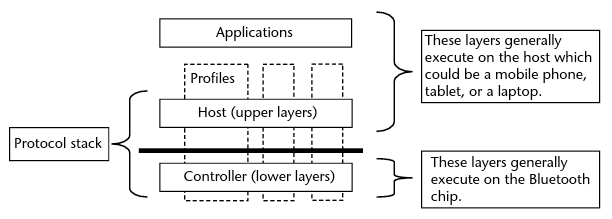
\includegraphics[width=0.8\textwidth]{images/bluetooth-architecture}
\caption{High-level architechture of Bluetooth. Illustration from \cite[p. 22]{gupta2013inside}.}
\label{fig:analysis:bluetooth:highlevel-architecture}
\end{figure}

As part of the upper layers, is the Logical Link Control and Adaption Protocol, abbreviated L2CAP. The protocol builds on top of protocols in the lower levels, to exchange data with a remote Bluetooth device. L2CAP provides functionality that includes segmentation and reassembly of packets, quality of service, streaming data and retransmission of packets. Devices communicating using L2CAP exchange PDU (Packet Data Unit) packets, containing information about the L2CAP protocol, e.g. the type of the PDU and a payload \cite[pp. 80-83]{gupta2013inside}. For example, the PDU type of a beacon can be \texttt{ADV\_NONCONN\_IND}, indicating a non-connectable undirected advertising packet. The payload of a PDU is referred to as the SDU (Service Data Unit) which originates from a level above the L2CAP, e.g. the Attribute Protocol \cite[p. 201]{gupta2013inside}.

Attribute Protocol, abbreviated ATT, uses L2CAP to transfer data. Mechanisms provided by ATT include discovering the attributes provided by a remote device and reading and writing the attributes. An attribute represents data, for example the temperature from a thermostat, the unit in which the temperature is provided or the name of a device. Attributes can be pushed or pulled to and from the a remote device. Attributes have a handle that identifies an attribute, a value and access permissions. The protocol works in a client-server manor in which a server expose a set of attributes and a client can read and write the attributes \cite{gupta2013inside}.

The Bluetooth Core 4.0 Specification, i.e. the specification including Bluetooth LE, introduces GATT profile architecture illustrated in \Cref{fig:analysis:bluetooth:gatt-architecture}. The GATT framework specifies how a device can discover, read, write, write and indicate its characteristics. Profiles consist of one or more services that are needed in order to provide a specific functionality, e.g. proximity monitoring \cite[p. 259-261]{gupta2013inside}. Services provide one or more characteristics that describe a feature, e.g. the temperature of a thermostat. Services may be shared by multiple profiles.

The Bluetooth Special Interest Group, the group maintaining the Bluetooth standards, provide a range of profiles, e.g. a proxmity profile for monitoring the distance to devices and a profile for heart rate sensors. Apple have developed the iBeacon profile for region monitoring and Google have developed the Eddystone profile for the same. Eddystone GATT profile defines the Eddystone Service that advertise \emph{frames} of information. These are described in detail in \Cref{sec:design:ble-positioning} as well as the Eddystone Configuration Services in which a device is connectable and the advertised values can be configured by a client BLE-enabled device.

\begin{figure}[!htb]
\centering
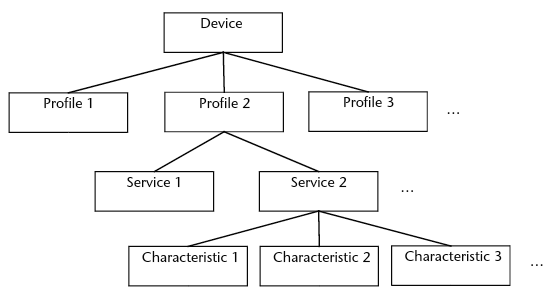
\includegraphics[width=0.8\textwidth]{images/gatt-architecture}
\caption{Relationship between profiles, services and characteristics. from \cite[p. 261]{gupta2013inside}.}
\label{fig:analysis:bluetooth:gatt-architecture}
\end{figure}

%%% Local Variables:
%%% mode: latex
%%% TeX-master: "../../master"
%%% End:
